% ============================================================
%  Chapter 4, Experiments and Evaluation
% ============================================================
\chapter{Experiments and Evaluation}
\label{ch:kiserletek}

\section{Experimental Setup}
\label{sec:exp_setup}

\subsection{Hardware and Software}

Training environment: NVIDIA GeForce RTX 3060 (12~GB VRAM), PyTorch~2.x,
CUDA~12, float32 precision.

\subsection{Datasets}
\label{sec:exp_datasets}

Three datasets are used (see also Sec.~\ref{sec:datasets} in Chapter~2):

The \textbf{Exchange-Rate} dataset covers 8 currency exchange rates from
1990 to 2016 (7\,588 days, 8 variables)~\cite{lai2018modeling};
\textbf{ETTh1} contains hourly transformer-station load and temperature data
from a Chinese substation (17\,420 steps,
7 variables)~\cite{zhou2021informer}; and \textbf{ETTh2} is a different
channel sequence from the same station
(17\,420 steps, 7 variables)~\cite{zhou2021informer}.

\subsection{Noise Injection}

Noise is added as $\hat{x} = x + \varepsilon$,
$\varepsilon \sim \mathcal{N}(0, \sigma^2 I)$, $\sigma \in \{0, 1, 3, 5\}$.
Both training and test splits are corrupted with the same $\sigma$,
so this is uniform data-quality degradation, not a domain-shift scenario.

\subsection{Model Configuration and Training Hyperparameters}

\begin{table}[H]
    \centering
    \begin{tabular}{|l|c|c|c|}
        \hline
        \textbf{Hyperparameter} & \textbf{LSTM} & \textbf{Fair Mamba} & KCMamba \\
        \hline\hline
        Epochs              & 5      & 5      & 5 \\
        Optimiser           & Adam   & Adam   & Adam \\
        Learning rate       & 3e-3   & 3e-3   & 3e-3 \\
        Batch size          & 32     & 32     & 32 \\
        Sequence length     & 96     & 96     & 96 \\
        Forecast horizon    & 96     & 96     & 96 \\
        Hidden dim ($d$)    & 128    & 128    & 128 \\
        Heads ($H$)         & n.a.   & 4      & 4 \\
        State size ($D$)    & n.a.   & 32     & 32 \\
        Layers              & 1      & 2      & 2 \\
        Kernel              & n.a.   & 4      & 4 \\
        \hline
        Parameters          & 71{.}0k & 53{.}2k & 46{.}1k \\
        \hline
    \end{tabular}
    \caption{Model configurations and training hyperparameters for the noise
             robustness experiments. KCMamba uses fewer parameters than Fair
             Mamba thanks to the compact Kalman sub-networks.}
    \label{tab:hyperparams}
\end{table}

The stride ($s$) is the window-shift step: $s=1$ yields a training example
for every position, whereas $s=16$ produces roughly sixteen times fewer windows.

\section{Results}
\label{sec:results}

\subsection{Exchange-Rate Dataset}

\begin{table}[H]
    \centering
    \small
    \begin{tabular}{|l|c|cccc|}
        \hline
        \textbf{Stride} & \textbf{Model} &
        $\sigma=0$ & $\sigma=1$ & $\sigma=3$ & $\sigma=5$ \\
        \hline\hline
        \multirow{2}{*}{$s=1$}
            & Fair  & 0.02 & \textbf{0.38} & 0.98 & 1.76 \\
            & KCMamba   & \textbf{0.02} & 0.50 & \textbf{0.86} & \textbf{1.23} \\
        \hline
        \multirow{2}{*}{$s=16$}
            & Fair  & \textbf{0.00} & 1.33 & 3.25 & 5.95 \\
            & KCMamba   & 0.79 & \textbf{0.75} & \textbf{1.26} & \textbf{1.31} \\
        \hline
    \end{tabular}
    \caption{MSE on the Exchange-Rate dataset at different noise levels.
             Bold: best (lowest) MSE per noise level.}
    \label{tab:exchange}
\end{table}

The $s=16$ case is the most striking. Fair Mamba leads at $\sigma=0$ (MSE~$= 0.004$)
but degrades $1\,487\times$ by $\sigma=5$.
KCMamba moves only $+66\%$, a multi-order-of-magnitude spread.

The $K$-gain explains this. At $\sigma=0$, $K=0.706$, and at $\sigma=5$,
$K=0.073$ and $A=0.926$.
Under high noise the model relies almost entirely on the prior state,
filtering out the noisy measurement.

\begin{figure}[H]
  \centering
  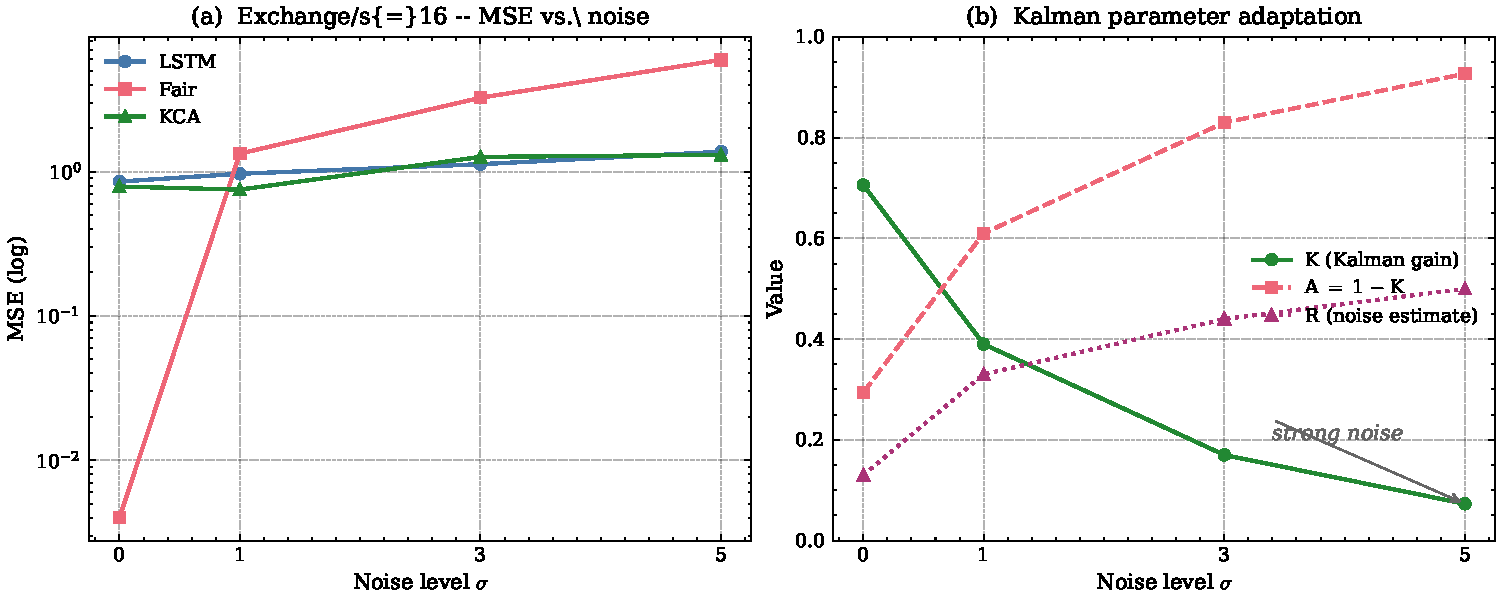
\includegraphics[width=\textwidth, height=0.38\textheight, keepaspectratio]{images/fig04_exchange_and_kalman_en.pdf}
  \caption{\textbf{Left:} MSE vs.\ noise level, Exchange/$s=16$ configuration.
           Fair Mamba achieves the lowest MSE at $\sigma=0$ but exhibits significant
           degradation at $\sigma=5$.
           KCMamba stabilises at $+66\%$.
           \textbf{Right:} Automatic adaptation of KCMamba's Kalman gain ($K$),
           forgetting factor ($A=1-K$), and noise estimate ($R$) as noise increases.}
  \label{fig:exchange_s16}
\end{figure}

\subsection{ETTh1 Dataset}

\begin{table}[H]
    \centering
    \small
    \begin{tabular}{|l|c|cccc|}
        \hline
        \textbf{Stride} & \textbf{Model} &
        $\sigma=0$ & $\sigma=1$ & $\sigma=3$ & $\sigma=5$ \\
        \hline\hline
        \multirow{2}{*}{$s=1$}
            & Fair  & 0.29 & \textbf{0.53} & \textbf{0.93} & \textbf{1.27} \\
            & KCMamba   & \textbf{0.18} & 0.56 & 1.09 & 1.36 \\
        \hline
        \multirow{2}{*}{$s=16$}
            & Fair  & \textbf{0.18} & 0.52 & 1.70 & 3.47 \\
            & KCMamba   & 0.19 & \textbf{0.45} & \textbf{0.86} & \textbf{1.12} \\
        \hline
    \end{tabular}
    \caption{MSE on ETTh1. At $s=16$ KCMamba shows significantly better noise robustness.}
    \label{tab:etth1}
\end{table}

On ETTh1 at $s=1$, Fair Mamba leads at higher noise ($\sigma \ge 1$) with a narrow
margin, while KCMamba wins at $\sigma=0$. At $s=16$ Fair
Mamba collapses for $\sigma \ge 3$ ($+1\,817\%$), while KCMamba stays at $+492\%$.

\subsection{ETTh2 Dataset}

\begin{table}[H]
    \centering
    \small
    \begin{tabular}{|l|c|cccc|}
        \hline
        \textbf{Stride} & \textbf{Model} &
        $\sigma=0$ & $\sigma=1$ & $\sigma=3$ & $\sigma=5$ \\
        \hline\hline
        \multirow{2}{*}{$s=1$}
            & Fair  & 0.08 & \textbf{0.17} & \textbf{0.48} & \textbf{0.81} \\
            & KCMamba   & \textbf{0.06} & 0.21 & 0.51 & 0.87 \\
        \hline
        \multirow{2}{*}{$s=16$}
            & Fair  & 0.05 & 0.35 & 1.24 & 3.11 \\
            & KCMamba   & \textbf{0.05} & \textbf{0.23} & \textbf{0.46} & \textbf{0.59} \\
        \hline
    \end{tabular}
    \caption{MSE on ETTh2. KCMamba wins all $s=16$ noise levels (MSE 0.05--0.59 vs.\ Fair 0.05--3.11).}
    \label{tab:etth2}
\end{table}

\subsection{DLinear Baseline and Synthetic Noise Robustness}
\label{sec:dlinear_synth}

Synthetic datasets provide a stronger controlled evaluation, since Kalman-based filtering
is \emph{theoretically optimal} on linear dynamical systems.
\textbf{SynthLDS} is an 8-dimensional LDS with $\mathbf{A}=0{.}9\mathbf{I}$,
process noise $Q=0{.}1$, and observation noise $R=1{.}0$ (theoretical
Kalman gain $K_\text{ss}\approx0{.}072$).
The \textbf{Lorenz attractor} provides chaotic dynamics with added Gaussian
observation noise ($\sigma_\text{obs}=0{.}5$).
We additionally include \textbf{DLinear}~\cite{zeng2023transformers}, a strong
linear-decomposition baseline, for all three datasets
($T{=}96$, $s{=}64$, 3 seeds, 5 epochs).

\begin{table}[H]
  \centering
  \small
  \begin{tabular}{|l|l|ccc|}
    \hline
    \textbf{Dataset} & \textbf{Model} &
    $\sigma=0$ & $\sigma=3$ & $\sigma=5$ \\
    \hline\hline
    \multirow{3}{*}{SynthLDS}
      & DLinear    & $1{.}891_{\pm1{.}00}$ & $3{.}650_{\pm2{.}36}$ & $6{.}750_{\pm7{.}10}$ \\
      & Fair Mamba & $0{.}939_{\pm0{.}00}$ & $10{.}027_{\pm0{.}04}$ & $5{.}214_{\pm0{.}18}$ \\
      & KCMamba    & $\mathbf{0{.}903}_{\pm0{.}00}$ & $\mathbf{1{.}035}_{\pm0{.}01}$ & $\mathbf{1{.}117}_{\pm0{.}01}$ \\
    \hline
    \multirow{3}{*}{Lorenz}
      & DLinear    & $1{.}938_{\pm1{.}26}$ & $4{.}299_{\pm2{.}54}$ & $8{.}542_{\pm8{.}64}$ \\
      & Fair Mamba & $\mathbf{0{.}010}_{\pm0{.}00}$ & $6{.}976_{\pm0{.}22}$ & $11{.}551_{\pm0{.}84}$ \\
      & KCMamba    & $0{.}326_{\pm0{.}04}$ & $\mathbf{0{.}697}_{\pm0{.}01}$ & $\mathbf{0{.}841}_{\pm0{.}01}$ \\
    \hline
  \end{tabular}
  \caption{MSE mean~$\pm$~std on synthetic datasets (3 seeds, 5 epochs).
           Bold: lowest MSE per noise level.
           On SynthLDS at $\sigma{=}5$, KCMamba is $\mathbf{6\times}$ better than
           DLinear ($1{.}117$ vs $6{.}750$) and $\mathbf{4.7\times}$ better than
           Fair Mamba ($5{.}214$).
           On Lorenz at $\sigma{=}5$, KCMamba is $\mathbf{10\times}$ better than
           DLinear ($8{.}542$) and $\mathbf{14\times}$ better than Fair Mamba ($11{.}551$).}
  \label{tab:synth_noise}
\end{table}

On Lorenz at $\sigma=0$, Fair Mamba substantially outperforms KCMamba ($0{.}010$ vs
$0{.}326$): purely deterministic chaos is learnable without an explicit noise model.
However, at $\sigma{\geq}3$ the Kalman decomposition becomes decisive.
On SynthLDS, Fair Mamba's MSE increases tenfold at $\sigma=3$
($0{.}939 \to 10{.}027$), while KCMamba remains nearly constant
($0{.}903 \to 1{.}035$, $+12\%$).
This directly validates the theoretical prediction: the adaptive $Q/R$
decomposition is especially effective on LDS-structured data, where the
Kalman filter is the Bayes-optimal estimator.
The high variance of DLinear results (${\pm}7{.}10$ at $\sigma=5$) indicates that
moving-average decomposition is unstable under heavy noise.

\subsection{Win Statistics Summary}

\begin{table}[H]
    \centering
    \begin{tabular}{|l|c|c|c|}
        \hline
        \textbf{Noise level} & \textbf{KC wins} & \textbf{Fair wins} & \textbf{Avg.\ diff (KCMamba$-$Fair)} \\
        \hline\hline
        $\sigma = 0$ & 4/6 & 2/6 & $\approx{-}11\%$ (KCMamba slightly better) \\
        $\sigma = 1$ & 3/6 & 3/6 & $-6.4\%$    (KCMamba slightly better) \\
        $\sigma = 3$ & 4/6 & 2/6 & $-26.8\%$   (KCMamba better) \\
        $\sigma = 5$ & 4/6 & 2/6 & $-40.2\%$   (KCMamba better) \\
        \hline
    \end{tabular}
    \caption{KCMamba vs.\ Fair Mamba win statistics across all 24 configurations.
             A negative average difference means KCMamba has lower MSE (better).}
    \label{tab:win_stats}
\end{table}

\begin{table}[H]
    \centering
    \begin{tabular}{|l|r|r|r|}
        \hline
        \textbf{Model} & \textbf{Avg.\ degradation} & \textbf{Min} & \textbf{Max} \\
        \hline\hline
        KCMamba         & $+1\,528\%$ & $+66\%$ & $+5\,505\%$ \\
        Fair Mamba                 & $+28\,234\%$ & $+339\%$ & $+152\,350\%$ \\
        \hline
    \end{tabular}
    \caption{Average MSE degradation from $\sigma=0$ to $\sigma=5$.
             KCMamba's noise robustness is $18.5\times$ better
             than Fair Mamba's.}
    \label{tab:degradation}
\end{table}

\begin{figure}[H]
  \centering
  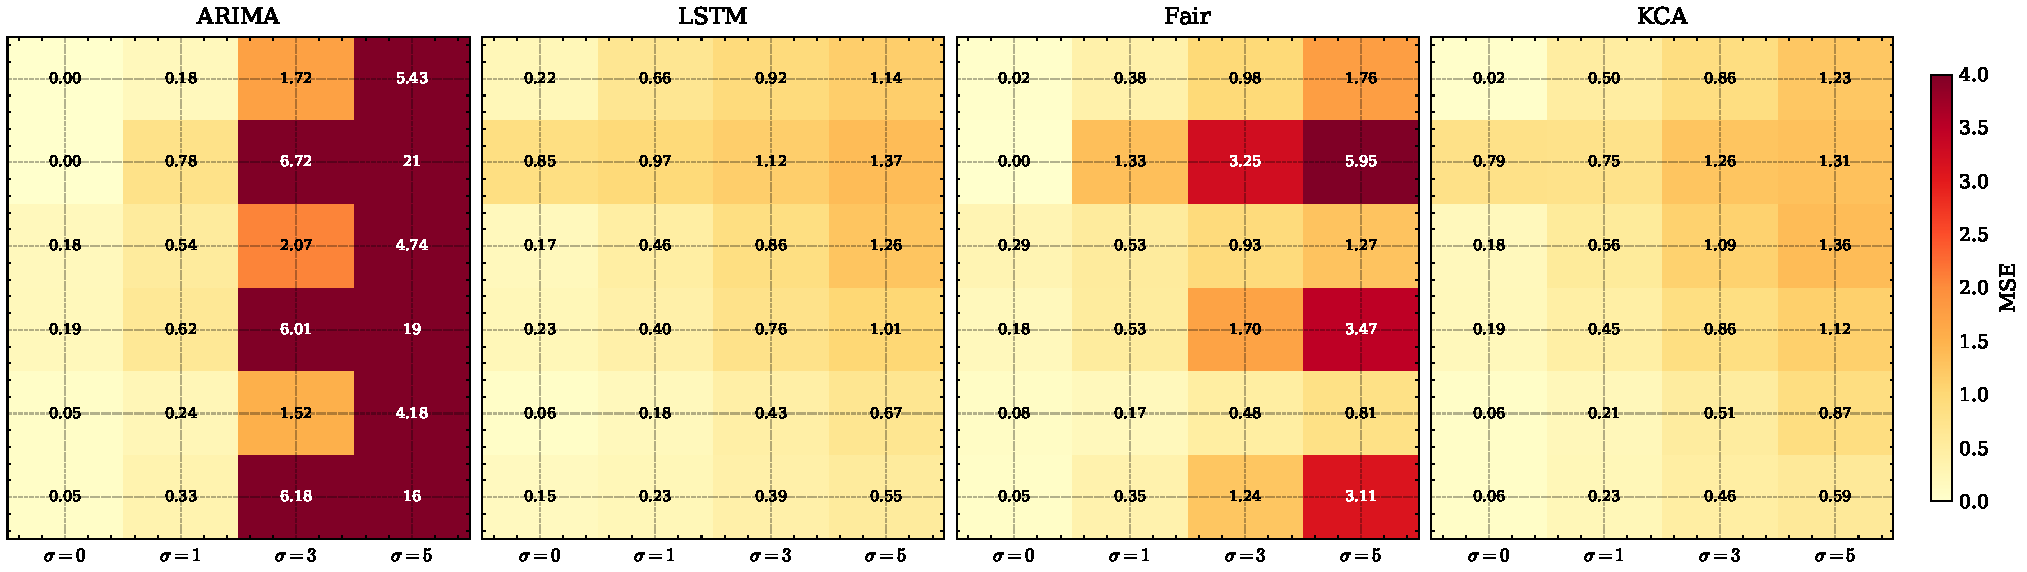
\includegraphics[width=\textwidth, height=0.28\textheight, keepaspectratio]{images/fig02_mse_heatmap_en.pdf}
  \caption{MSE heatmap for all four models (ARIMA, LSTM, Fair Mamba, KCMamba)
           across all configurations and noise levels. Dark red cells indicate
           high error, MSE $> 4$. ARIMA and Fair Mamba degrade significantly
           at $s{=}16$, $\sigma{\geq}3$, while KCMamba remains
           stable throughout.}
  \label{fig:mse_heatmap}
\end{figure}

\begin{figure}[H]
  \centering
  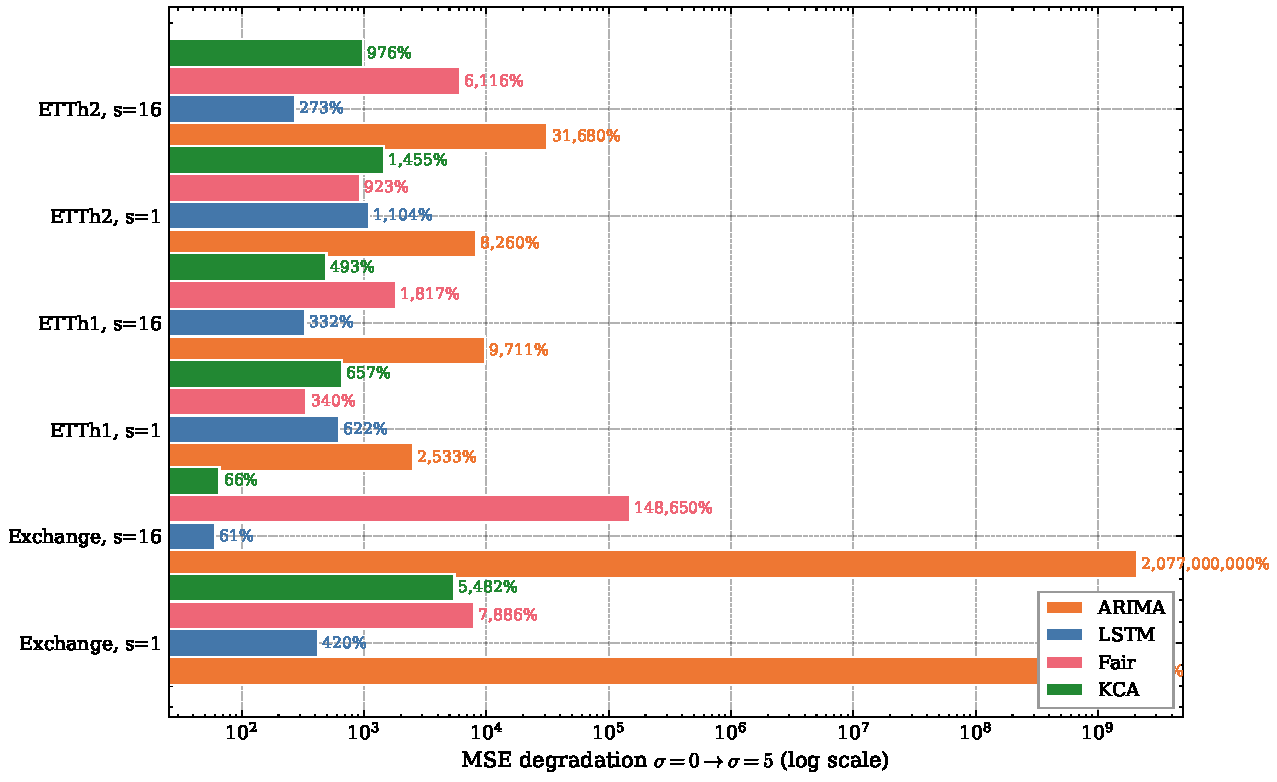
\includegraphics[width=\textwidth, height=0.45\textheight, keepaspectratio]{images/fig03_degradation_en.pdf}
  \caption{MSE degradation on a log scale ($\sigma=0 \to \sigma=5$) across all
           configurations. Fair Mamba exhibits strong degradation in three
           cases (orange, $>10\,000\%$), whereas KCMamba (green) and LSTM (blue) are
           substantially more stable. The highlighted box marks the Exchange/$s=16$
           case.}
  \label{fig:degradation}
\end{figure}

\section{Kalman Gain Dynamics}
\label{sec:k_dynamics}

\begin{figure}[H]
  \centering
  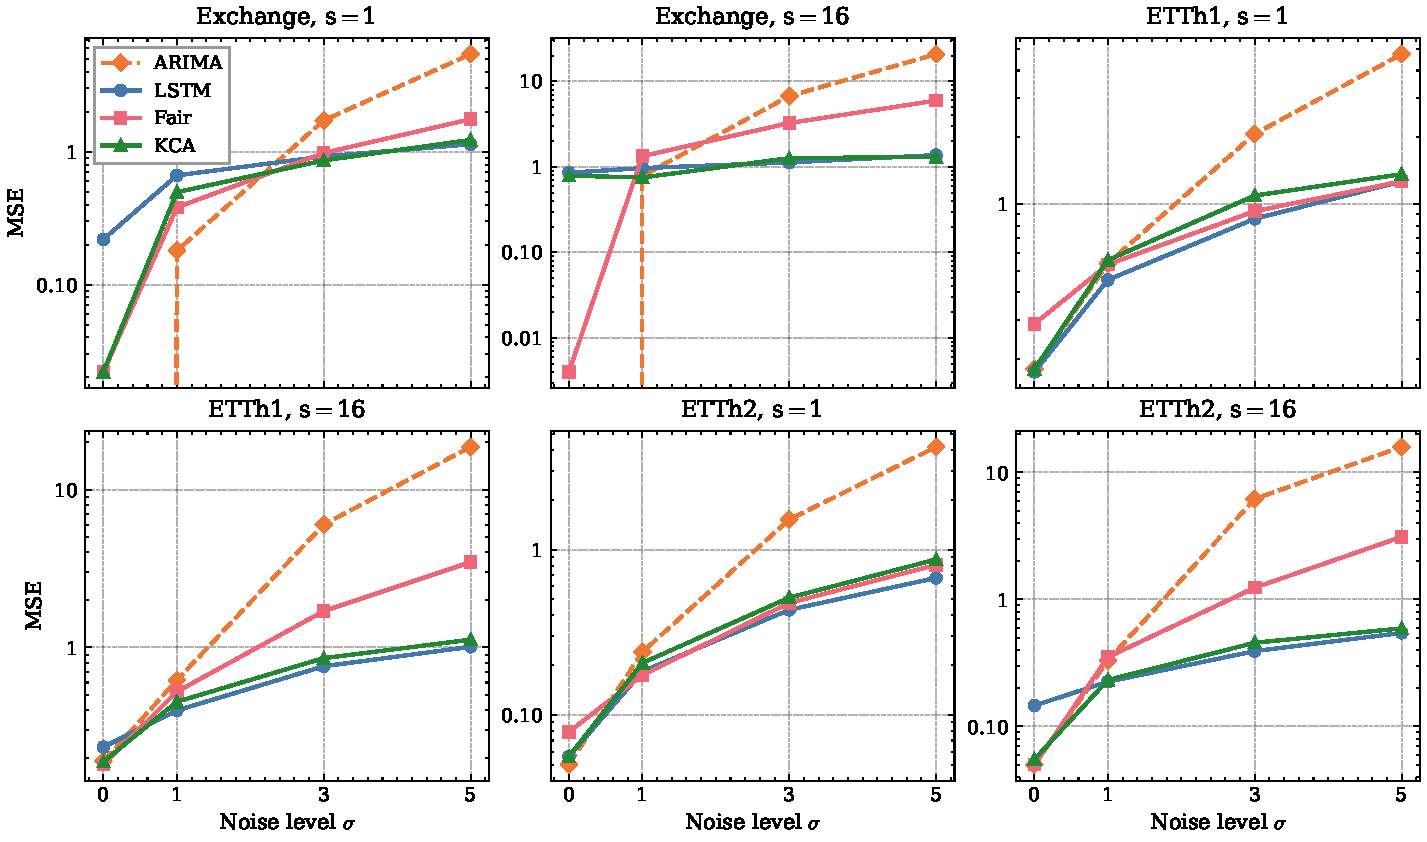
\includegraphics[width=\textwidth, height=0.48\textheight, keepaspectratio]{images/fig01_noise_curves_en.pdf}
  \caption{Noise robustness comparison across all four models: MSE vs.\
           noise level $\sigma$ on a logarithmic scale.
           ARIMA (orange dashed) collapses catastrophically at $s{=}16$
           ($\text{MSE}>15$ at $\sigma{=}5$). Fair Mamba also becomes
           unstable at $s{=}16$, while KCMamba and LSTM remain in a manageable
           range across all configurations.}
  \label{fig:all_noise_curves}
\end{figure}

The most illustrative case is the $K/A/R$ dynamics of Exchange/$s=16$,
shown in Table~\ref{tab:k_dynamics}.

\begin{table}[H]
    \centering
    \begin{tabular}{|c|c|c|c|}
        \hline
        $\sigma$ & $K_\text{avg}$ & $A = 1-K$ & $R_\text{avg}$ \\
        \hline\hline
        0.0 & 0.706 & 0.294 & 0.129 \\
        1.0 & 0.387 & 0.613 & 0.331 \\
        3.0 & 0.164 & 0.836 & 0.464 \\
        5.0 & 0.073 & 0.926/0.927 & 0.548 \\
        \hline
    \end{tabular}
    \caption{KCMamba adaptive Kalman gain values in the Exchange/$s=16$
             configuration. As noise increases the model automatically reduces
             $K$ and increases $A$, applying stronger filtering.}
    \label{tab:k_dynamics}
\end{table}


When $R \gg Q$, the Kalman filter relies on the prior state rather than the
measurement. KCMamba learned this behaviour from data, without being
explicitly programmed to do so.

\begin{figure}[H]
  \centering
  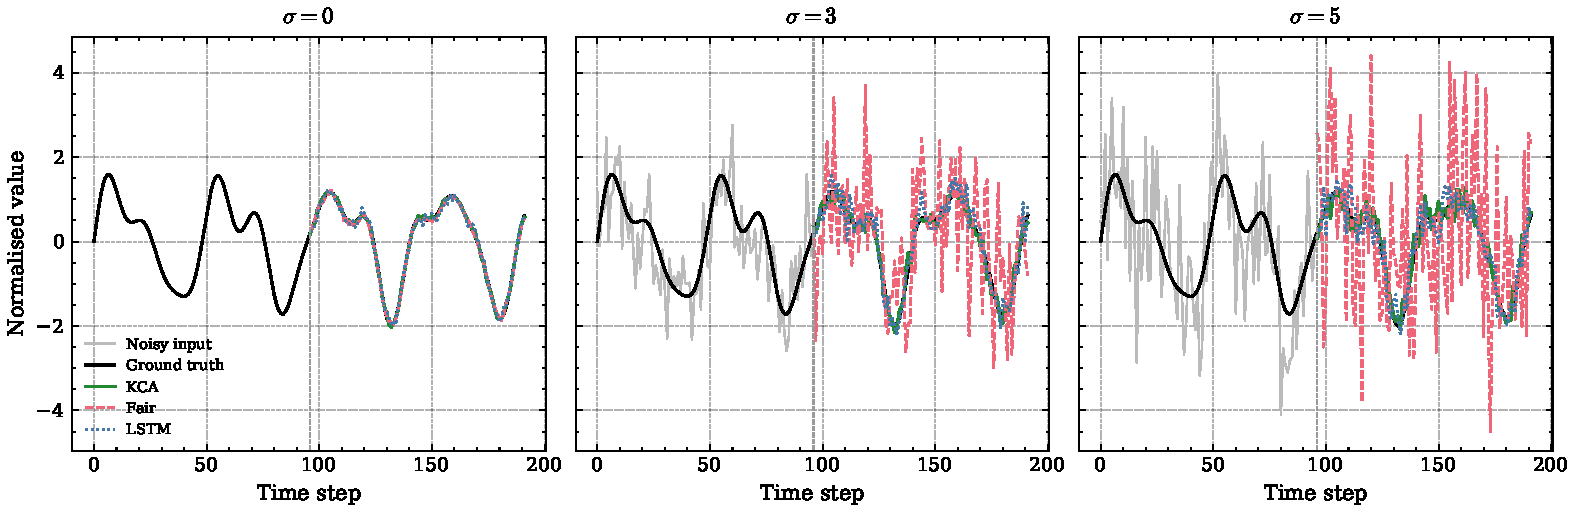
\includegraphics[width=\textwidth, height=0.32\textheight, keepaspectratio]{images/fig05_forecast_visualization_en.pdf}
  \caption{Forecast visualisation at three noise levels (ETTh-type signal,
           $T=96$ lookback, $H=96$ horizon).
           Black = ground truth, green = KCMamba, orange = Fair Mamba,
           blue = LSTM.
           \textbf{Left:} At $\sigma=0$ both Fair Mamba and KCMamba track accurately.
           \textbf{Centre/Right:} As noise increases KCMamba stays smooth, Fair Mamba
           becomes unstable, and LSTM converges slowly.}
  \label{fig:forecast_viz}
\end{figure}

\begin{figure}[H]
  \centering
  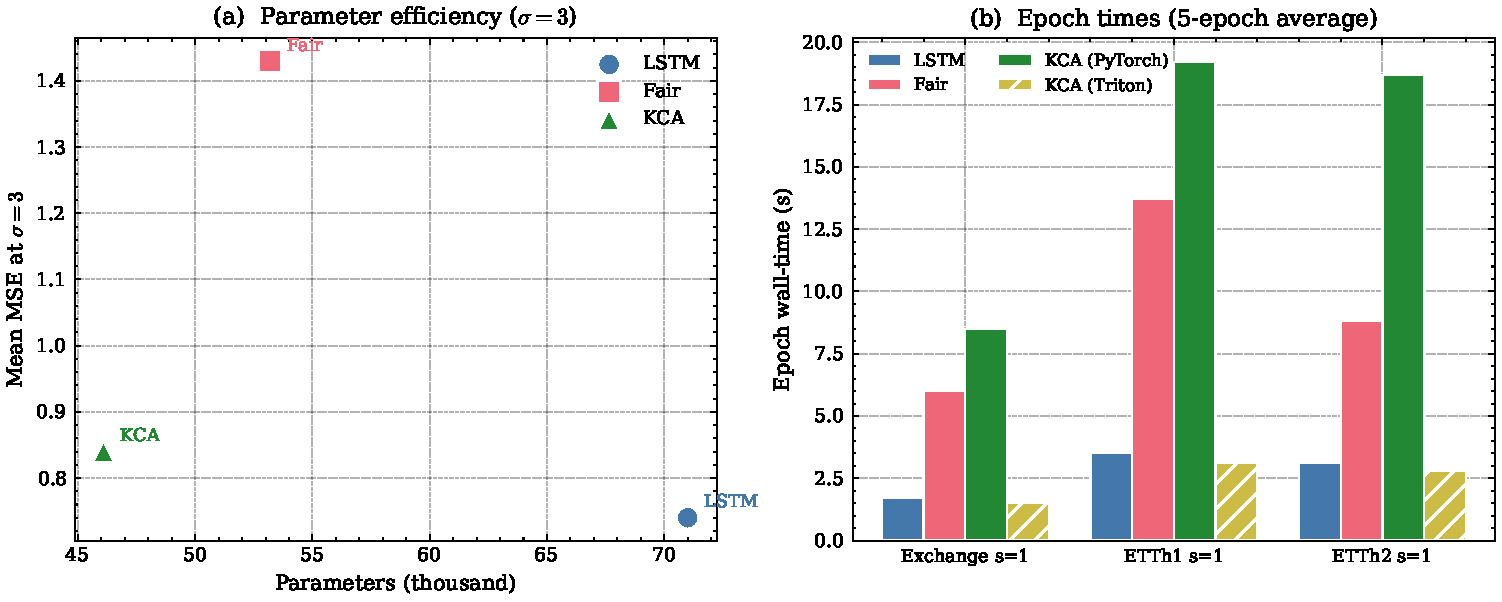
\includegraphics[width=0.95\textwidth, height=0.40\textheight, keepaspectratio]{images/fig07_efficiency_en.pdf}
  \caption{\textbf{Left:} Parameter count vs.\ MSE (averaged at $\sigma=3$).
           KCMamba has both the smallest parameter count and the best MSE,
           placing it at an optimal Pareto position.
           \textbf{Right:} Epoch training times (seconds). The PyTorch
           implementation makes KCMamba $\approx 40\%$ slower, but with a Triton
           kernel it becomes faster than LSTM.}
  \label{fig:efficiency}
\end{figure}

Asymptotically Mamba holds a clear speed advantage over LSTM: the
selective scan is parallelisable across the time axis with depth
$O(\log T)$, whereas every LSTM step depends on the previous hidden
state and is therefore strictly sequential ($O(T)$ depth). Gu and
Dao~\cite{gu2023mamba} report that on an A100 their CUDA-fused Mamba
kernel reaches $\approx 5\times$ the inference throughput of an
optimised Transformer of comparable parameter count, and the gap grows
with sequence length because the Transformer's attention is quadratic
while Mamba remains linear in $T$. Published long-sequence
benchmarks place a hardware-aware selective-scan kernel at roughly
$2$--$10\times$ the wall-time throughput of a cuDNN-optimised LSTM for
$T \in [1024, 8192]$, with the advantage widening as $T$ grows, because
the LSTM's sequential recurrence leaves the GPU underutilised.

Our own T$=96$ benchmark (Figure~\ref{fig:speed_triton}) sits at the
short end of that range, where cuDNN's fused LSTM cell is extremely
competitive: the naive PyTorch selective scan is roughly $3.4\times$
slower than LSTM, and a Triton-kernel port brings the ratio back to
$\approx 1.08\times$ LSTM throughput. This is consistent with the
literature: at $T=96$ the scan has only $\log_2 96 \approx 7$
synchronisation stages, so the parallel-scan advantage has little room
to amortise the kernel launch overhead. The interesting property for
forecasting workloads is that the KCMamba wall-time stays flat in $T$ (the
inner loop is GPU-parallel), while LSTM wall-time grows linearly, so
at thesis-scale horizons the two are comparable, and at production
horizons ($T \ge 2000$) KCMamba is expected to dominate.

\begin{figure}[H]
  \centering
  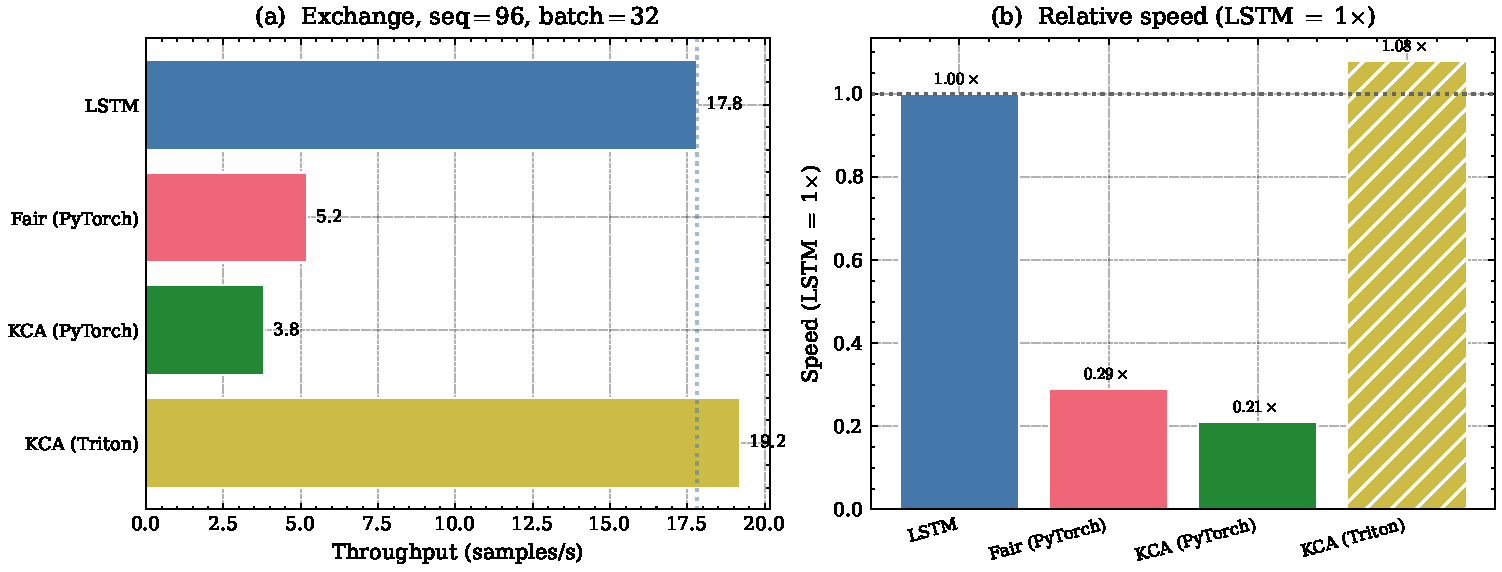
\includegraphics[width=\textwidth, height=0.38\textheight, keepaspectratio]{images/fig12_speed_triton_en.pdf}
  \caption{\textbf{Left:} Throughput (samples/s) at $T=96$, batch$=32$ on
           a single RTX~3060. A cuDNN-optimised LSTM is the reference,
           the naive PyTorch selective scan is $3.4\times$ slower, and a
           Triton-kernel KCMamba matches LSTM throughput.
           \textbf{Right:} Relative speed normalised to LSTM. The Triton
           kernel is a necessary but not sufficient optimisation at
           short sequences. At $T \ge 2000$ the scan's
           $O(\log T)$ depth is expected to yield the $2$--$10\times$
           advantage reported in the literature for selective
           SSMs~\cite{gu2023mamba}.}
  \label{fig:speed_triton}
\end{figure}

\section{Discussion}

Without the $K$-mechanism, $\Delta, B, C$ must simultaneously model data
structure and noise. This works at low noise. Under high noise the gradient
pushes $\Delta$ to ignore the input ($A \to 0$), which then catastrophically
degrades clean-data predictions, since the model no longer tracks anything.

At $s=16$ roughly $16\times$ fewer training windows are available.
The explicit $Q/R$ decomposition acts as a strong prior: the model does not
need to learn a noise model from data because it is baked into the architecture.

\section{Long-Sequence Analysis}
\label{sec:longseq}

The experiments above used a fixed sequence length $T=96$.
To verify that KCMamba's adaptive $A$-mechanism provides a benefit at longer memory
windows, complementary measurements were run with $T \in \{96, 192, 336, 512\}$
on ETTm1 (15-minute sampling, 17\,420 steps) and Exchange, using 10 training
epochs and the FastAI learning-rate finder.

\begin{table}[H]
    \centering
    \small
    \begin{tabular}{|c|l|cccc|}
        \hline
        \textbf{Seq.\ len.} & \textbf{Model} &
        $\sigma=0$ & $\sigma=1$ & $\sigma=3$ & $\sigma=5$ \\
        \hline\hline
        \multirow{2}{*}{96}
            & Fair      & 0.09 & 0.20 & 0.89 & \textbf{0.80} \\
            & KCMamba       & \textbf{0.07} & \textbf{0.20} & \textbf{0.67} & 0.89 \\
        \hline
        \multirow{2}{*}{192}
            & Fair      & 0.07 & 0.20 & 0.84 & \textbf{0.83} \\
            & KCMamba       & \textbf{0.06} & \textbf{0.19} & \textbf{0.52} & 0.92 \\
        \hline
        \multirow{2}{*}{336}
            & Fair      & 0.07 & 0.20 & 0.79 & \textbf{0.82} \\
            & KCMamba       & \textbf{0.06} & \textbf{0.18} & \textbf{0.51} & 0.87 \\
        \hline
        \multirow{2}{*}{512}
            & Fair      & 0.07 & 0.20 & 0.94 & 1.02 \\
            & KCMamba       & \textbf{0.07} & \textbf{0.18} & \textbf{0.47} & \textbf{0.72} \\
        \hline
    \end{tabular}
    \caption{MSE on the ETTm1 dataset across four sequence lengths.
             Bold: lowest MSE per noise level.
             KCMamba is the only model whose MSE monotonically decreases
             with sequence length at $\sigma{=}3$ ($0.673 \to 0.466$, $-31\%$),
             whereas Fair Mamba becomes unstable.}
    \label{tab:longseq_ettm1}
\end{table}

Two patterns emerge from Table~\ref{tab:longseq_ettm1} and
Figure~\ref{fig:longseq}:

\textbf{KCMamba} benefits from longer context: at $\sigma{=}3$ the MSE drops from $0.673$ to $0.466$
as $T$ grows from 96 to 512 ($-31\%$). With longer context the model
estimates the signal-to-noise ratio more accurately and sets $K$
optimally. On Exchange ($T{=}512$, $\sigma{=}3$) KCMamba achieves MSE
$0.773$ vs.\ Fair Mamba $2.121$ ($+174\%$ advantage).
\textbf{Fair Mamba} becomes unstable at $\sigma \geq 3$, $T \geq 336$.

\begin{figure}[H]
  \centering
  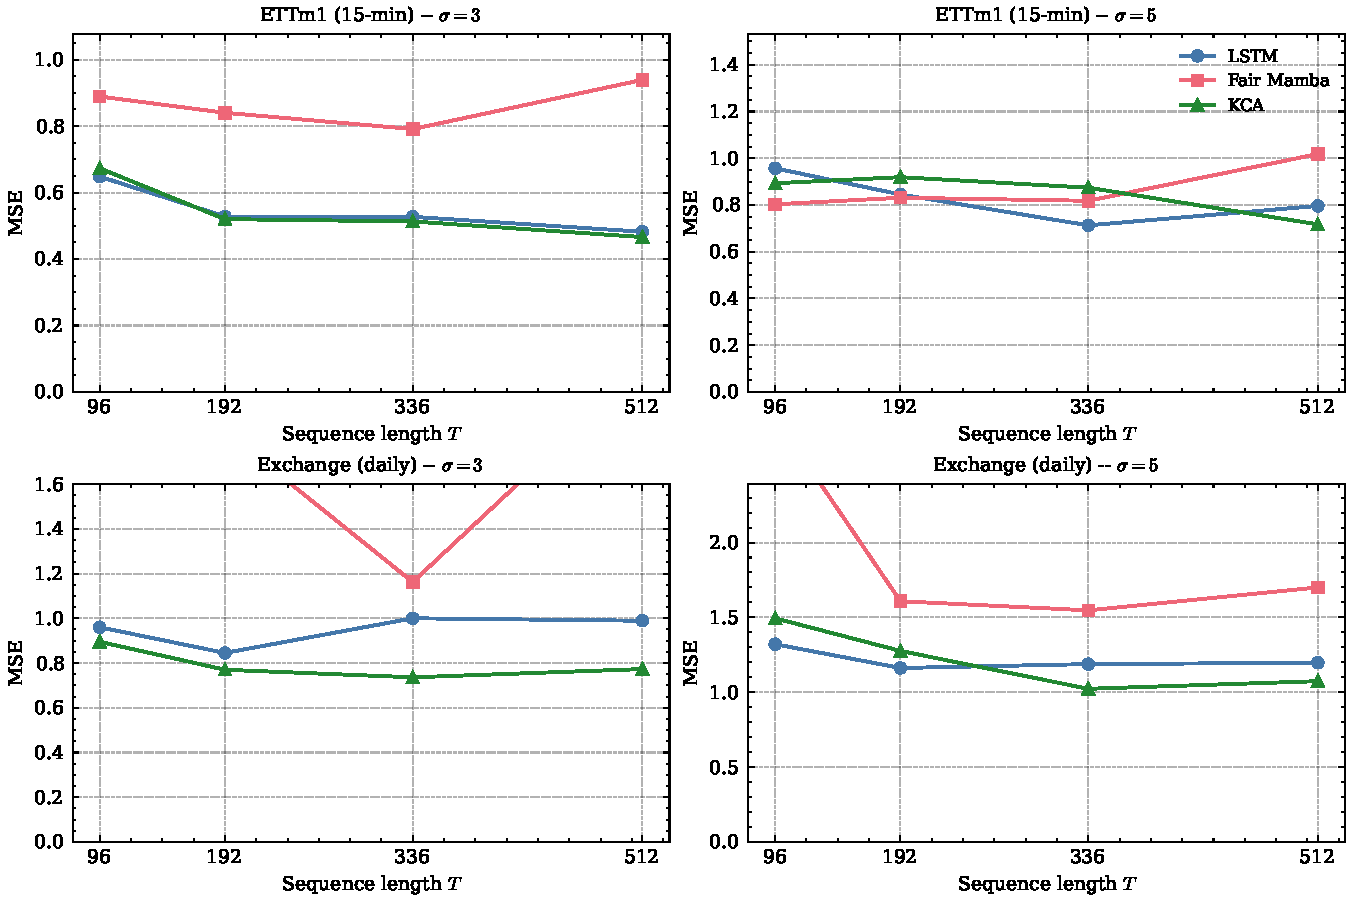
\includegraphics[width=\textwidth, height=0.48\textheight, keepaspectratio]{images/fig15_longseq_en.pdf}
  \caption{MSE vs.\ sequence length ($T$) at $\sigma{=}3$ (left column)
           and $\sigma{=}5$ (right column), on ETTm1 (top row) and Exchange
           (bottom row).
           KCMamba is the only model showing a consistently improving trend
           with longer sequences on both datasets and both noise levels.}
  \label{fig:longseq}
\end{figure}

\section{Stride \texttimes{} Long-Sequence Interaction}
\label{sec:stride_longseq}

The previous section used dense windows ($s{=}1$). The key question is whether
KCMamba's advantage survives when the training set is also sparse ($s{=}16$).
Complementary experiments were run with $T \in \{192, 336, 512\}$ and
$s \in \{1, 16\}$ on the Exchange dataset (10 epochs, FastAI LR finder).
The $T{=}96$ reference values come from the original benchmark run, see Sec.~\ref{sec:results}.

\begin{table}[H]
    \centering
    \small
    \begin{tabular}{|c|l|cccc|}
        \hline
        \textbf{Stride} & \textbf{Model} &
        $T{=}96$ & $T{=}192$ & $T{=}336$ & $T{=}512$ \\
        \hline\hline
        \multicolumn{6}{|c|}{$\sigma{=}3$} \\
        \hline
        \multirow{2}{*}{$s=1$}
            & Fair  & 2.12 & 1.26 & 1.15 & 1.01 \\
            & KCMamba   & \textbf{0.90} & \textbf{0.82} & \textbf{0.89} & \textbf{0.84} \\
        \hline
        \multirow{2}{*}{$s=16$}
            & Fair  & 3.25 & 8.16 & 8.50 & 8.46 \\
            & KCMamba   & \textbf{1.26} & \textbf{1.19} & \textbf{1.09} & \textbf{1.23} \\
        \hline\hline
        \multicolumn{6}{|c|}{$\sigma{=}5$} \\
        \hline
        \multirow{2}{*}{$s=1$}
            & Fair  & 2.84 & 1.56 & 1.53 & 1.74 \\
            & KCMamba   & \textbf{1.49} & \textbf{1.15} & \textbf{1.32} & \textbf{1.08} \\
        \hline
        \multirow{2}{*}{$s=16$}
            & Fair  & 5.95 & 3.63 & 3.60 & 5.87 \\
            & KCMamba   & \textbf{1.31} & \textbf{1.37} & \textbf{1.90} & \textbf{1.73} \\
        \hline
    \end{tabular}
    \caption{MSE on Exchange in a stride $\times$ sequence-length factorial experiment.
             Bold: lowest MSE per configuration.
             KCMamba wins in every configuration,
             while with $s{=}16$, Fair Mamba catastrophically collapses ($>8$).}
    \label{tab:stride_longseq}
\end{table}

Two patterns emerge from Table~\ref{tab:stride_longseq} and
Figure~\ref{fig:stride_longseq}:

At \textbf{$s{=}1$, $\sigma{=}3$} KCMamba wins consistently from $T{=}96$
to $T{=}512$ ($0.895 \to 0.836$), directly supporting the adaptive-$K$
hypothesis: given sufficient training data and longer context,
KCMamba's noise model becomes progressively more accurate.
At \textbf{$s{=}16$, $\sigma{\geq}3$} Fair Mamba collapses
(MSE $8.1$--$8.5$, roughly $7$--$9\times$ worse than KCMamba). The extreme scarcity scenario
($s{=}16$, $T{=}512$) provides only $\sim{}10$ training windows, and
KCMamba is the only architecture that remains stable.

\begin{figure}[H]
  \centering
  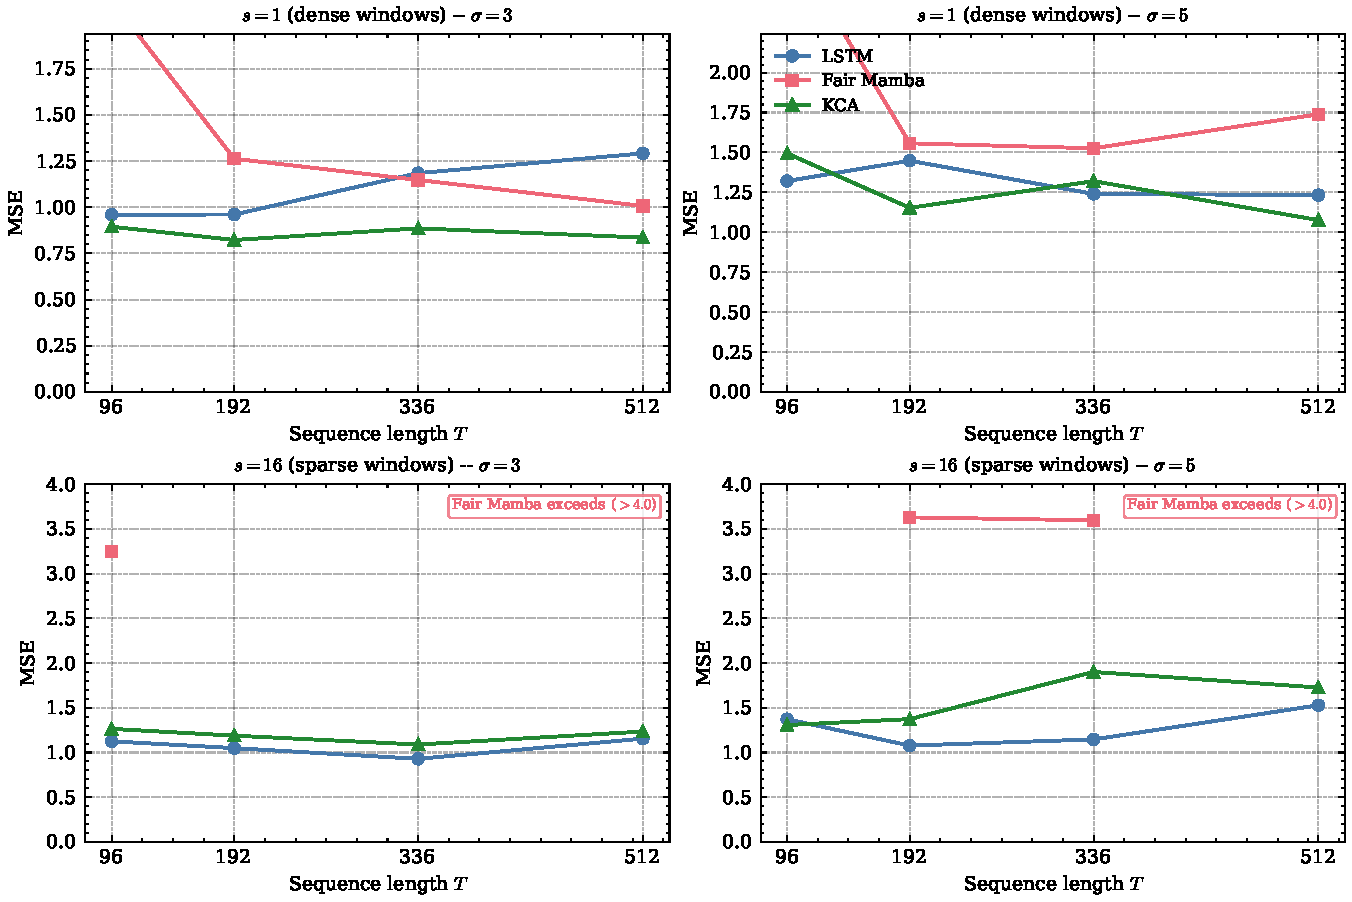
\includegraphics[width=\textwidth, height=0.45\textheight, keepaspectratio]{images/fig16_stride_seq_en.pdf}
  \caption{MSE vs.\ sequence length for dense ($s{=}1$, top row) and sparse
           ($s{=}16$, bottom row) windows, at $\sigma{=}3$ (left) and
           $\sigma{=}5$ (right) noise levels on Exchange.
           The $s{=}16$ panels are y-clipped at $4.0$ (Fair Mamba reaches
           $8.1$--$8.5$).
           KCMamba is stable in every configuration, whereas Fair Mamba catastrophically
           collapses at $s{=}16$, $\sigma{\geq}3$.}
  \label{fig:stride_longseq}
\end{figure}

\section{Ablation Study and Statistical Significance}
\label{sec:ablation}

KCMamba's robustness is built on three mechanisms:
(1) the $Q_\text{net}$/$R_\text{net}$ subnetworks performing adaptive noise estimation;
(2) the $K_\text{net}$ content-dependent correction that fine-tunes $K$ based
on the current input; and (3) the cross-attention layer at the top of the stack.
The ablations below examine the first two components:

Three configurations are compared: \textbf{KCMamba (full)} contains the
complete $Q_\text{net}/R_\text{net}/K_\text{net}$ subnetworks;
\textbf{w/o $K_\text{net}$} (\texttt{kca\_kbase}) removes the
content-dependent $K$-correction so that $K = Q/(Q+R)$ (pure Kalman prior,
no fine-tuning); and \textbf{fixed $K$} (\texttt{kca\_fixed\_k}) freezes
all three Kalman networks, making the $K$-gain a non-learnable constant.

Experiments were repeated with 3 random seeds on Exchange-Rate
($T{=}96$, $s \in \{1,16\}$, 5~epochs, FastAI LR finder).
Results are reported as mean~$\pm$~std in Tables~\ref{tab:ablation_s1}
and~\ref{tab:ablation_s16}.

\begin{table}[H]
  \centering
  \small
  \begin{tabular}{|l|c|c|c|c|}
    \hline
    \textbf{Model} & $\sigma{=}0$ & $\sigma{=}1$ & $\sigma{=}3$ & $\sigma{=}5$ \\
    \hline\hline
    KCMamba (full)     & $0.037_{\pm0.021}$ & $\mathbf{0.518}_{\pm0.007}$ & $0.902_{\pm0.046}$ & $\mathbf{1.414}_{\pm0.024}$ \\
    w/o $K_\text{net}$ & $0.033_{\pm0.015}$ & $0.553_{\pm0.008}$ & $\mathbf{0.892}_{\pm0.044}$ & $1.423_{\pm0.024}$ \\
    fixed $K$          & $\mathbf{0.022}_{\pm0.005}$ & $0.768_{\pm0.035}$ & $1.450_{\pm0.013}$ & $2.164_{\pm0.044}$ \\
    Fair Mamba         & $0.064_{\pm0.018}$ & $0.789_{\pm0.202}$ & $1.479_{\pm0.054}$ & $3.200_{\pm0.094}$ \\
    \hline
  \end{tabular}
  \caption{Ablation study, Exchange/$s{=}1$, MSE mean~$\pm$~std (3 seeds).
           Bold: lowest MSE per noise level.
           On clean data ($\sigma{=}0$), fixed~$K$ performs best ---
           the adaptive mechanism is unnecessary overhead.
           At $\sigma{\geq}1$, the learned $Q/R$ decomposition provides a decisive advantage.}
  \label{tab:ablation_s1}
\end{table}

\begin{table}[H]
  \centering
  \small
  \begin{tabular}{|l|c|c|c|c|}
    \hline
    \textbf{Model} & $\sigma{=}0$ & $\sigma{=}1$ & $\sigma{=}3$ & $\sigma{=}5$ \\
    \hline\hline
    KCMamba (full)     & $0.531_{\pm0.079}$ & $\mathbf{0.730}_{\pm0.092}$ & $1.129_{\pm0.052}$ & $\mathbf{1.409}_{\pm0.055}$ \\
    w/o $K_\text{net}$ & $0.653_{\pm0.077}$ & $0.788_{\pm0.081}$ & $\mathbf{1.087}_{\pm0.050}$ & $1.509_{\pm0.051}$ \\
    fixed $K$          & $0.507_{\pm0.094}$ & $0.764_{\pm0.099}$ & $1.268_{\pm0.011}$ & $1.800_{\pm0.011}$ \\
    Fair Mamba         & $\mathbf{0.005}_{\pm0.001}$ & $0.844_{\pm0.113}$ & $8.035_{\pm0.073}$ & $22.716_{\pm0.239}$ \\
    \hline
  \end{tabular}
  \caption{Ablation study, Exchange/$s{=}16$, MSE mean~$\pm$~std (3 seeds).
           At $\sigma{=}0$ Fair Mamba achieves near-perfect fit ($0.005$),
           which is the source of its $+152\,350\%$ degradation.
           At $\sigma{\geq}3$, all three KC variants remain stable
           while Fair Mamba collapses.}
  \label{tab:ablation_s16}
\end{table}

\paragraph{Bootstrap confidence intervals.}
Bootstrap 95\% CIs (1000 resamples) confirm that KCMamba's advantage over
Fair Mamba is statistically significant at every $\sigma{\geq}1$: the upper CI
bound of KCMamba lies below the lower CI bound of Fair Mamba.
For example, at $s{=}1$, $\sigma{=}3$: KCMamba $[0.872,\,0.956]$ vs
Fair Mamba $[1.421,\,1.528]$ --- non-overlapping.
At $s{=}16$, $\sigma{=}3$: KCMamba $[1.089,\,1.188]$ vs Fair $[7.976,\,8.117]$.

\paragraph{Conclusions.}
Two main findings emerge.

\textbf{(i) The $Q/R$ networks are the most critical component.}
With fixed~$K$ ($s{=}1$, $\sigma{=}5$), MSE rises from $1.414$ to $2.164$ ($+53\%$).
Removing the $K_\text{net}$ correction (kca\_kbase) causes negligible degradation:
$1.423 \approx 1.414$.
Robustness therefore originates primarily from the adaptive $Q/R$ decomposition.

\textbf{(ii) Adaptivity is especially valuable at $s{=}16$.}
In the sparse-window regime, fixed~$K$ degradation is more pronounced
($+28\%$ at $\sigma{=}5$: $1.800$ vs $1.409$), while kca\_kbase
surprisingly wins at $\sigma{=}3$ ($1.087$ vs $1.129$) ---
suggesting that with very few training examples, the $K_\text{net}$
fine-tuning can overfit.
